% !TEX root = ../../thesis.tex

% \newpage
% \thispagestyle{plain}
% \mbox{}
% 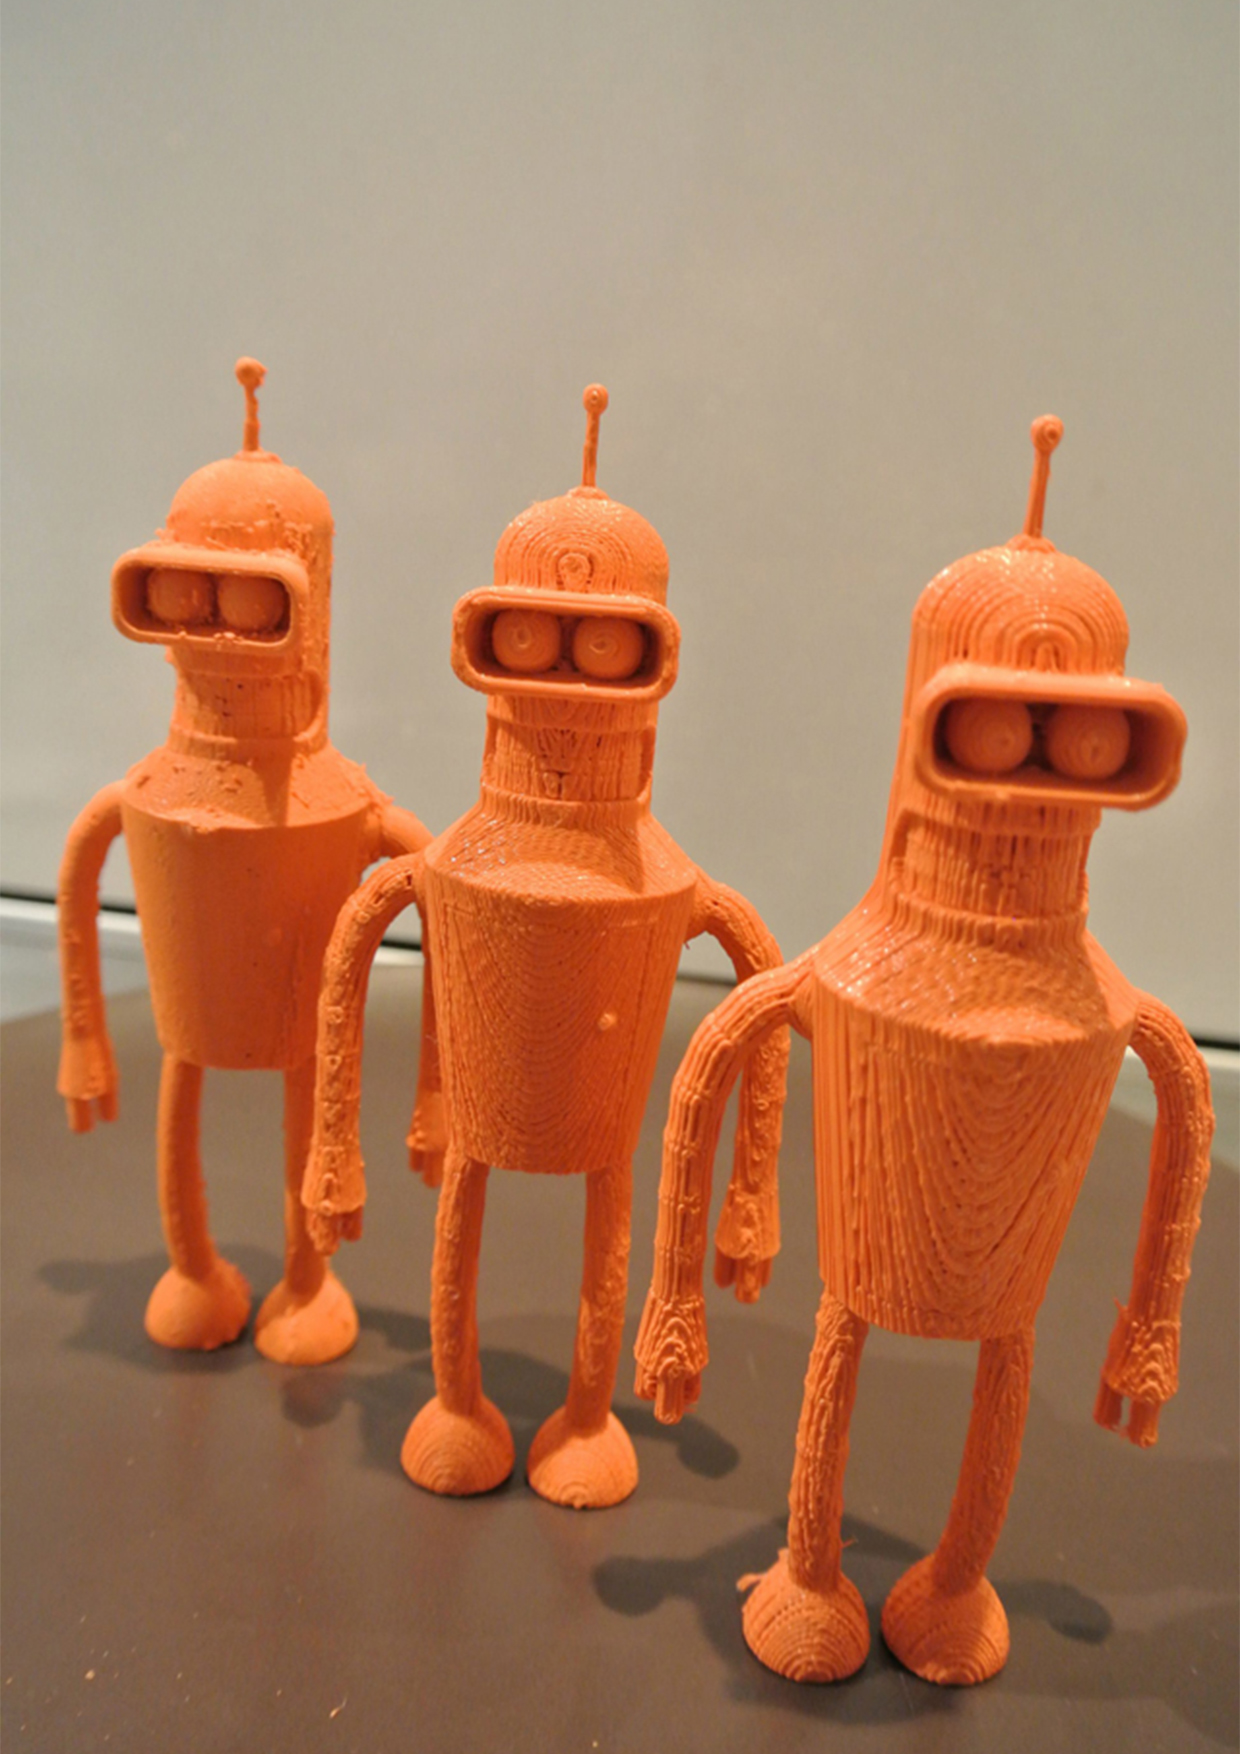
\includepdf{/Users/matthieulapeyre/Documents/phd_thesis/media/3DprintedBlender.pdf}

\chapter{The open hardware and 3D printing revolution}

% \cleanchapterquote{third industrial revolution}{the economist}

\section{Introduction} % (fold)

With the democratization of personal computers and the development of Internet, computer science and application have know a great expansion. Open source software played a major role, indeed most of the web are running under Linux operating system and Apache while open source software like Qt, openGL, openCL, OpenCV, and so on permitted the realization of a wide variety of daily life applications.

However while copying and sharing bits of a software is virtually free and can often be run on any computer, producing the atoms of a real object both has a potentially high cost and requires expert tooling. Thus the production of mechanic or electronic hardware components is limited to two options: either it is handcrafted or mass produced. Also the step between handcrafted prototype and mass production is so high only big company can reach it. Conventional manufacturing processes requires the production of specific tools, the programming of complex machine, the human intervention to put the part along the different tool and so on, most of the cost are in the up-front tooling, and the more complicated a product is, the more it costs. Thus, most of companies will not accept to run a whole production process just for few units and if they accept the cost will be so high than most prototypes never find a way to reach people outside the workshop they had been created. So until now, production in small or medium series was extremely difficult to achieve because it was not profitable.
Only big companies were able to raise enough money to produce new hardware and the niche products and personalization were left aside.

Since few years, a novel evolution, also predicted to become the next industrial revolution~\cite{anderson} is going to completely change the current rules of the production.

The way we build and the way we share

In this chapter, we will discuss the emergence of new production tools also coming with new way to share work.

\section{The 3D printing revolution} % (fold)

A comparison of rapid prototyping technologies (Pham 1997)

"Prototyping is an essential part of the product development and manugacturing cycle required for assessing the forim, fit and functionality of a design before a significant investment in tooling is made.
Until recently, prototypes were largerly handmade by skilled craftsmen, adding weeks or months to the product development time.
Because of this, only a few design iterations could be made before tooling went into production, resulting in parts which at best were seldom optimised and at worst did not function properly.
Rapid Prototyping is a term which embraces a range of new technologies for producing accurate parts directly from CAD models in a few hours, with littel need for human intervention.
This means that desigenrs have the freedom to produce physical models of theirs drawings more frequently, allowing them to check the assembly and function of the design as well as discussing downstream manufacturing issues with an easy-to-interpret, unambigous prototype.
Consequently, errors are minimised and product development costs and lead times substantially reduced.
It has been claimed that rapid proto can cut new product costs by up to 70\% and the time to market by 90\%."
- Rapid product development in the USA, Europe and Japan (Waterman 1994)

3D printing is any of various processes of making a three-dimensional object from a numeric model (mainly 3D) primarily through additive processes in which successive layers of material are laid down under computer control.

\subsection{Several available techniques} % (fold)

\subsubsection{Stereolithography (SL)} % (fold)

This relies on a photosensitive monomer resin which forms a polymer and solidifies when exposed to ultraviolet (UV) light.
Due to the absorption and scattering of the beam this reaction only takes place near the surface.

Y'en a plein dans A comparison of rapid prototyping technologies (Pham 1997)

\subsubsection{Selective laser sintering} % (fold)
SLS uses a fine powder which is heated with a CO2 laser of power in the range of 25-50W such that the surface tensions of the grains are overcome and they fuse together.Before the powder is sintered, the entire bed is headted to just below the melting point of the material in order to minimize thermal distortion and facilitate fusion to the previous layer.

\subsubsection{Filament} % (fold)

\subsection{Totaly revolution the design process} % (fold)

\subsection{Expected major impact in the day to come} % (fold)

The SuperDraco differs from most rocket engines in that its combustion chamber is 3D printed by direct metal laser sintering (DMLS), where complex metal structures are printed by using a laser to build the object out of metal powders one thin layer at a time. The regeneratively-cooled combustion chamber is made of inconel; a family of nickel-chromium alloy that’s notable for its high strength and toughness, and is also used in the Falcon 9’s Merlin engine.

“Through 3D printing, robust and high-performing engine parts can be created at a fraction of the cost and time of traditional manufacturing methods,” says Elon Musk, Chief Designer and CEO at SpaceX. “SpaceX is pushing the boundaries of what additive manufacturing can do in the 21st century, ultimately making our vehicles more efficient, reliable and robust than ever before.”

As 3D printers became more accessible to consumers, online social platforms have developed to support the community.[131] This includes websites that allow users to access information such as how to build a 3D printer, as well as social forums that discuss how to improve 3D print quality and discuss 3D printing news, as well as social media websites that are dedicated to share 3D models.[132][133][134] RepRap is a wiki based website that was created to hold all information on 3d printing, and has developed into a community that aims to bring 3D printing to everyone. Furthermore, there are other sites such as Thingiverse, which was created initially to allow users to post 3D files for anyone to print, allowing for decreased transaction cost of sharing 3D files. These websites have allowed for greater social interaction between users, creating communities dedicated around 3D printing.


\paragraph{A comparison of rapid prototyping technologies (Pham 1997)}

"Prototyping is an essential part of the product development and manugacturing cycle required for assessing the forim, fit and functionality of a design before a significant investment in tooling is made.
Until recently, prototypes were largerly handmade by skilled craftsmen, adding weeks or months to the product development time.
Because of this, only a few design iterations could be made before tooling went into production, resulting in parts which at best were seldom optimised and at worst did not function properly.
Rapid Prototyping is a term which embraces a range of new technologies for producing accurate parts directly from CAD models in a few hours, with littel need for human intervention.
This means that desigenrs have the freedom to produce physical models of theirs drawings more frequently, allowing them to check the assembly and function of the design as well as discussing downstream manufacturing issues with an easy-to-interpret, unambigous prototype.
Consequently, errors are minimised and product development costs and lead times substantially reduced.
It has been claimed that rapid proto can cut new product costs by up to 70\% and the time to market by 90\%."
- Rapid product development in the USA, Europe and Japan (Waterman 1994)




\section{The open hardware movement} % (fold)

The concept of "open-source hardware" or "open hardware" is not yet as well known or widespread as the free software or open-source software concept. However, it shares the same principles: anyone should be able to see the source (the design documentation in case of hardware), study it, modify it and share it.

The emergence of new and accessible rapid prototyping techniques change the way to produce things. Because it is now quick, simple and cheap to make things, it opens the realm of possibility to share hardware because anyone can produce it. Open source hardware is now making sense and is currently exponentially expanding.

\subsection{History} % (fold)
- Machine à soie de Lyon.

- Homebrew computing club
\subsection{Open Hardware definition} % (fold)

The Open Source Hardware Association (OSHWA) aims to be the voice of the open hardware community. It promotes the use and development of open source hardware for education and economic development, collect, compile and publish data on the open source movement and organize the movement around shared and principles.

Also the Open Source Hardware Association defines\footnote{Complete definition available on \url{http://www.oshwa.org/definition/}.} the open source hardware as:

\begin{row}{4}{2}
    \begin{cell}{3}
        \emph{Hardware whose design is made publicly available so that anyone can study, modify, distribute, make, and sell the design or hardware based on that design. The hardware’s source, the design from which it is made, is available in the preferred format for making modifications to it. Ideally, open source hardware uses readily-available components and materials, standard processes, open infrastructure, unrestricted content, and open-source design tools to maximize the ability of individuals to make and use hardware. Open source hardware gives people the freedom to control their technology while sharing knowledge and encouraging commerce through the open exchange of designs.}
    \end{cell}
    \begin{cell}{1}
        \begin{NFfigure}
            \centering
                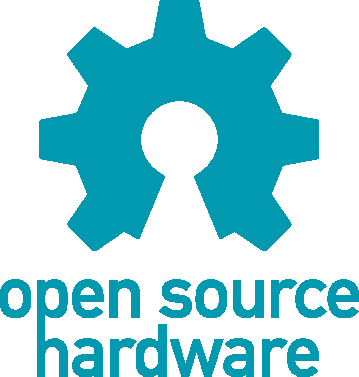
\includegraphics[height=4cm]{oshw-logo.pdf}
            \caption{The open source hardware logo}
            \label{fig:ohw-logo}
        \end{NFfigure}
    \end{cell}
\end{row}


\subsection{Open source hardware licenses} % (fold)

The Open Source Hardware Association definition is not enough, a legal framework is needed to both protect and promote open hardware project. This is the role of the open source licenses which will be discussed in this section.

In general, there are two broad classes of open-source licenses: copyleft and permissive. Copyleft licenses (sometimes referred to as “viral”) are those which require derivative works to be released under the same license as the original; common copyleft licenses include the GNU General Public License (GPL) and the Creative Commons Attribution-ShareAlike license. Other copyleft licenses have been specifically designed for hardware; they include the CERN Open Hardware License (OHL) and the TAPR Open Hardware License (OHL). Permissive licenses are those which allow for proprietary (closed) derivatives; they include the FreeBSD license, the MIT license, and the Creative Commons Attribution license


\subsubsection{Creative Commons licenses} % (fold)
\begin{row}{4}{2}
    \begin{cell}{3}
        Founded in 2001, Creative Commons is a nonprofit organization that enables the sharing and use of creativity and knowledge through free legal tools. They provide a free and understandable licenses standardizing the way to share and use creative work. Thanks to the use of several modules which can be combined, the Creative Commons licenses permit to the creator to modify his copyright terms to best suit his needs. First intended for artistic and cultural content such as music and writing, the Creative Commons are now used also to share open source harware files.
    \end{cell}
    \begin{cell}{1}
        \begin{NFfigure}
            \centering
                
\includegraphics[height=3cm]{cc-logo.png}
            \caption{Creative Commons logo}
            \label{fig:cc_logo}
        \end{NFfigure}
    \end{cell}
\end{row}
The Creative Commons licenses are based on four major condition modules:
\begin{description}
    \item[Attribution (BY)]: requiring attribution to the original author.
    \item[Non Commercial (NC)]: requiring the work is not used for commercial purposes
    \item[No Derivative works (ND)]: allowing only the original work, without derivatives
    \item[Share Alike (SA)]: allowing derivative works under the same or a similar license (later or jurisdiction version).
\end{description}


The combination of these modules leads to six licenses (see \figurename~\ref{fig:all-cc-licenses}) but related to the open only two of them are considered as open source following the OSHW definition:
\begin{description}
    \item[Attribution CC BY] People can distribute, remix, tweak and build upon the licensed work, even commercially, as long as they credit the authors of the original creation.
    \item[Attribution-ShareAlike CC BY-SA] People can distribute, remix, tweak and build upon the licensed work, even commercially, as long as they credit the authors and license their new creations under the identical terms. \textbf{This license is often compared to “copyleft” free and open source software licenses.}
\end{description}

\begin{figure}[]
    \begin{center}
        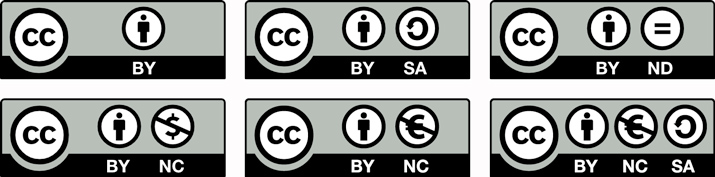
\includegraphics[width=0.8\linewidth]{all-cc-licenses.jpg}
    \end{center}
    \caption{The combination of the 4 Creative Commons modules give 6 licenses allowing creators to choose how they want to share their work and how "open" they are.}
    \label{fig:all-cc-licenses}
\end{figure}

\subsubsection{CERN OHL} % (fold)

Inspired by the open source software movement, the Open Hardware Repository\footnote{\url{http://www.ohwr.org/}} was created to enable hardware developers to share the results of their R\&D activities. The recently published (mars 2013) CERN Open Hardware Licence offers the legal framework to support this knowledge and technology exchange.

The CERN–OHL is to hardware what the General Public Licence (GPL) is to software. It defines the conditions under which a licensee will be able to use or modify the licensed material and is compliant with the OSHWA definition criteria. In the spirit of knowledge sharing and dissemination, the CERN Open Hardware Licence (CERN OHL) governs the use, copying, modification and distribution of hardware design documentation, and the manufacture and distribution of products\footnote{License details available on \url{http://www.ohwr.org/projects/cernohl/wiki}}.


\subsubsection{TAPR Open Hardware License (OHL)}
Specifically designed for open hardware, and avoids the issues other licenses have with focusing on copyright protecting documentation instead of the right to make, distribute, or use a product based on that documentation. Requires that all derived works use the same license and include before and after documentation if any changes were made.

Visit the TAPR website for the full text of the TAPR Open Hardware License (OHL). The numbered sections of the agreement take precedence over this preamble.


\subsection{Some famous open hardware projects} % (fold)


\subsubsection{Arduino} % (fold)

Students from the Interaction Design Institute Ivrea in Italy were using \emph{BASIC Stamp}\footnote{A BASIC Stamp module is a single-board computer that runs the Parallax PBASIC language interpreter in its microcontroller.} for a cost of \$100.

\begin{row}{4}{2}
    \begin{cell}{3}
      Started in 2005 by Banzi and al., the Arduino project aimed to offer an affordable and easy to use electronics board for student-friendly price: \$30. The first wiring design was done during the phd thesis of Hernando Barragan~\cite{barragan2004wiring}. After the wiring platform was complete, researchers worked to make it lighter, less expensive, and available to the open source community.
    \end{cell}
    \begin{cell}{1}
        \begin{NFfigure}
            \centering
                
\includegraphics[height=2.5cm]{arduino_logo.png}
            \caption{The Arduino logo}
            \label{fig:arduino_logo}
        \end{NFfigure}
    \end{cell}
\end{row}

\begin{quotation}
  Arduino is a platform for prototyping interactive objects using electronics. It consists of both hardware and software: a circuit board that can be purchased at low cost or assembled from freely-available plans; and an open-source development environment and library for writing code to control the board. Arduino comes from a philosophy of learning by doing and strives to make it easy to work directly with the medium of interactivity. It extends the principles of open source to the realm of hardware, supporting a community of people working with and extending the platform. It has been used in universities around the world and in numerous works of interactive art.

  \signed{Mellis~\cite{mellis2007arduino}}
\end{quotation}

The arduino story was one of the first hardware project with a real desire to promote the innovation trough open source, to make it work they had to find an appropriate licensing solution that could apply to their board. After some investigation, they realized that if they simply looked at their project differently, (i.e. considering the source files as documentation\footnote{\emph{"You could think of hardware as piece of culture you want to share with other people"}, Banzi. }), they could use a license from Creative Commons normally used for cultural works such as music and writing.

Today, Arduino is a very successful project. The boards and derivatives are used by hundreds of thousands people and a lot of project from all domains would not possible if Arduino have not existed, among them Poppy.


\subsection{Shapeoko}

Designed by Edward Ford, Shapeoko (see \figurename~\ref{fig:shapeoko}) is a simple, low cost (\$685) and open source (CC BY-SA)CNC milling machine. It is based on two other open hardware projects: MakerSlide\footnote{Open source linear bearing system under Creative Common BY-SA licenses: \url{http://makerslide.com/}} for linear motion and an Arduino board for the control.

\begin{figure}[]
    \begin{center}
        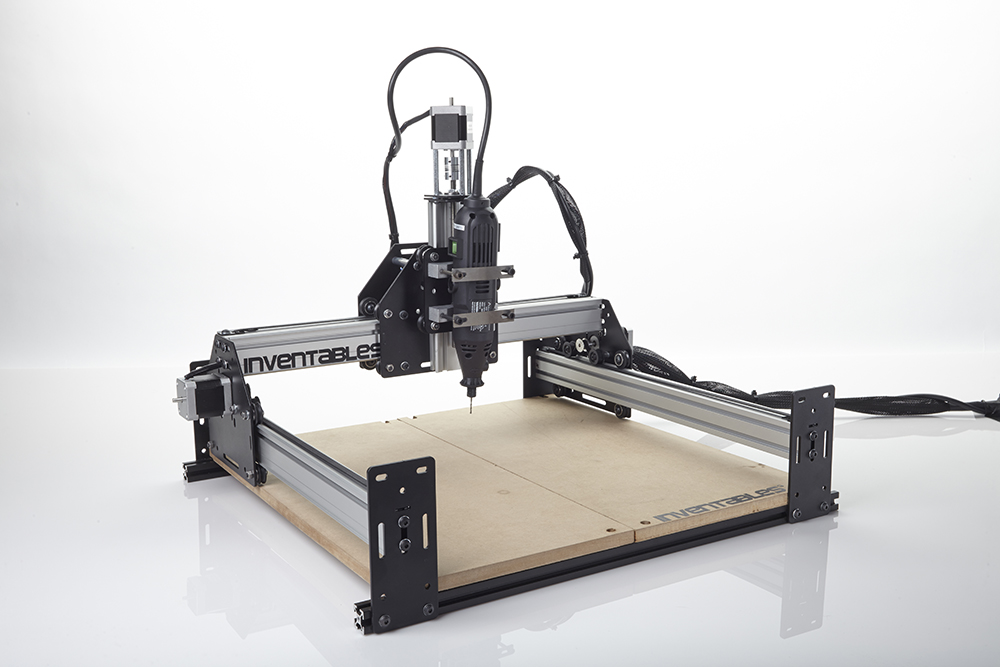
\includegraphics[width=0.8\linewidth]{shapeoko_v2.jpg}
    \end{center}
    \caption{The shapeoko v2 is a low cost and open source CNC 2.5 axes.}
    \label{fig:shapeoko}
\end{figure}

\subsubsection{RepRap} % (fold)

The RepRap project started in 2005 and based on the Fab@Home\footnote{\url{http://www.fabathome.org/}} principles, developped a multi-proposed open source 3D printer using Fused Deposition Modeling\footnote{TODO}(FFD) technique with the particularity to be largerly self-replicating:

\begin{quotation}
    RepRap is an open-source self-replicating rapid prototyping machine. It is a robot that uses fused-filament fabrication1 to make engineering components and other products from a variety of thermoplastic polymers. RepRap has been designed to be able automatically to print out a significant fraction of its own parts. All its remaining parts have been selected to be standard engineering materials and components available cheaply worldwide. As the machine is free and open-source anyone may – without royalty payments – make any number of copies of it ether for themselves or for others, using RepRap machines themselves to reproduce those copies.

    \signed{~\cite{jones2011reprap}}
\end{quotation}


\begin{figure}[]
\centering
    \subfloat[][RepRap v2]{\label{fig:RepRap_v2}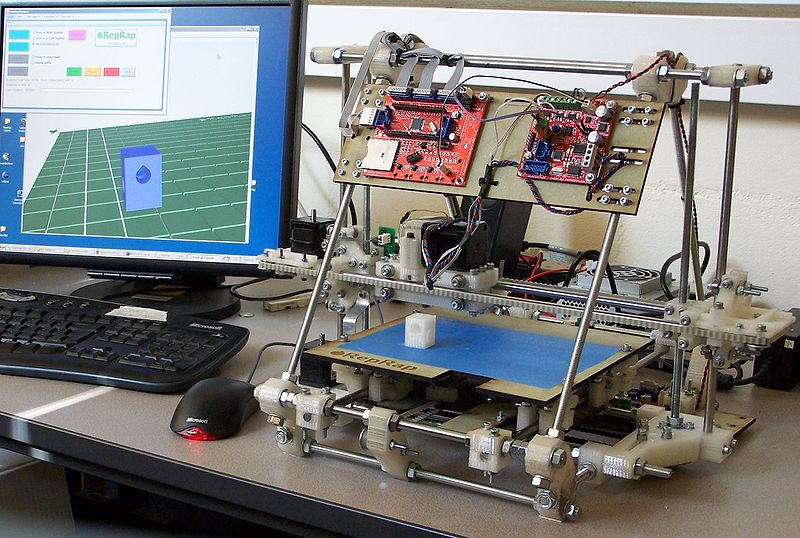
\includegraphics[width=0.45\linewidth]{RepRap_v2.jpg}}
    \hfil
    \subfloat[][MakerBot Replicator v1]{\label{fig:makerbot-replicator}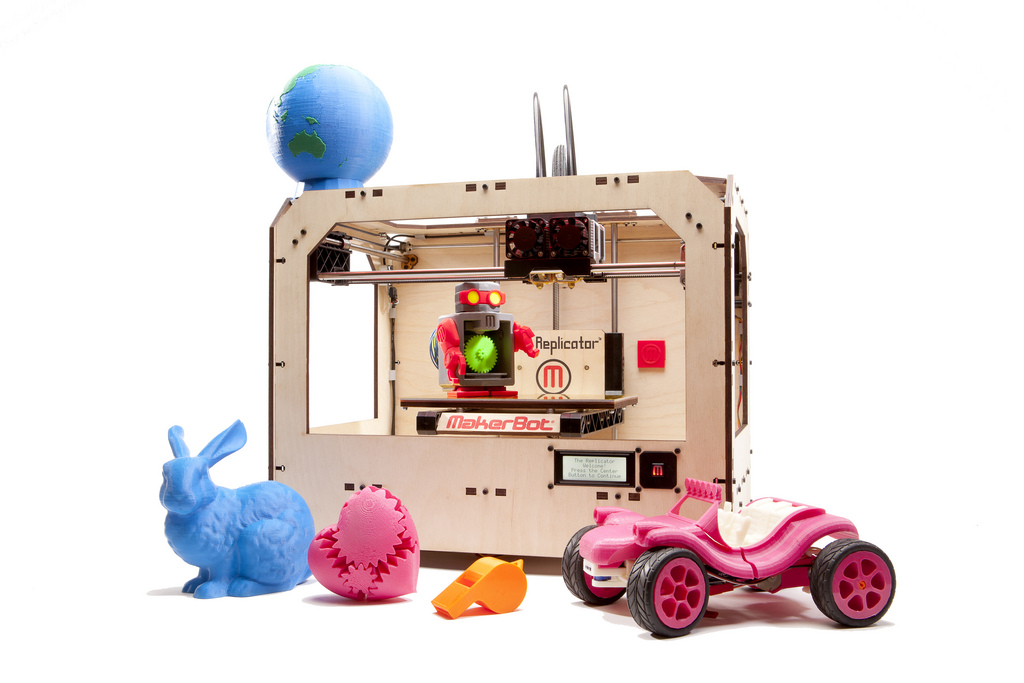
\includegraphics[width=0.45\linewidth]{makerbot-replicator.jpg}}
    \caption{}
    \label{fig:RepRap_project}
\end{figure}


Distributed under GNU General Public License, the RepRap (see \figurename~\ref{fig:RepRap_v2}) was one of the first low-cost 3D printer. The fact it is genuinely collaborative, this project generated a so large number of variations and interpretations that is even difficult to count (see \figurename~\ref{fig:RepRap_family_tree}). One of them is the now famous Makerbot Replicator (see \figurename~\ref{fig:makerbot-replicator}). Now Makerbot is one of the major worldwide general public 3D printer distributor.

\begin{figure}[]
    \begin{center}
        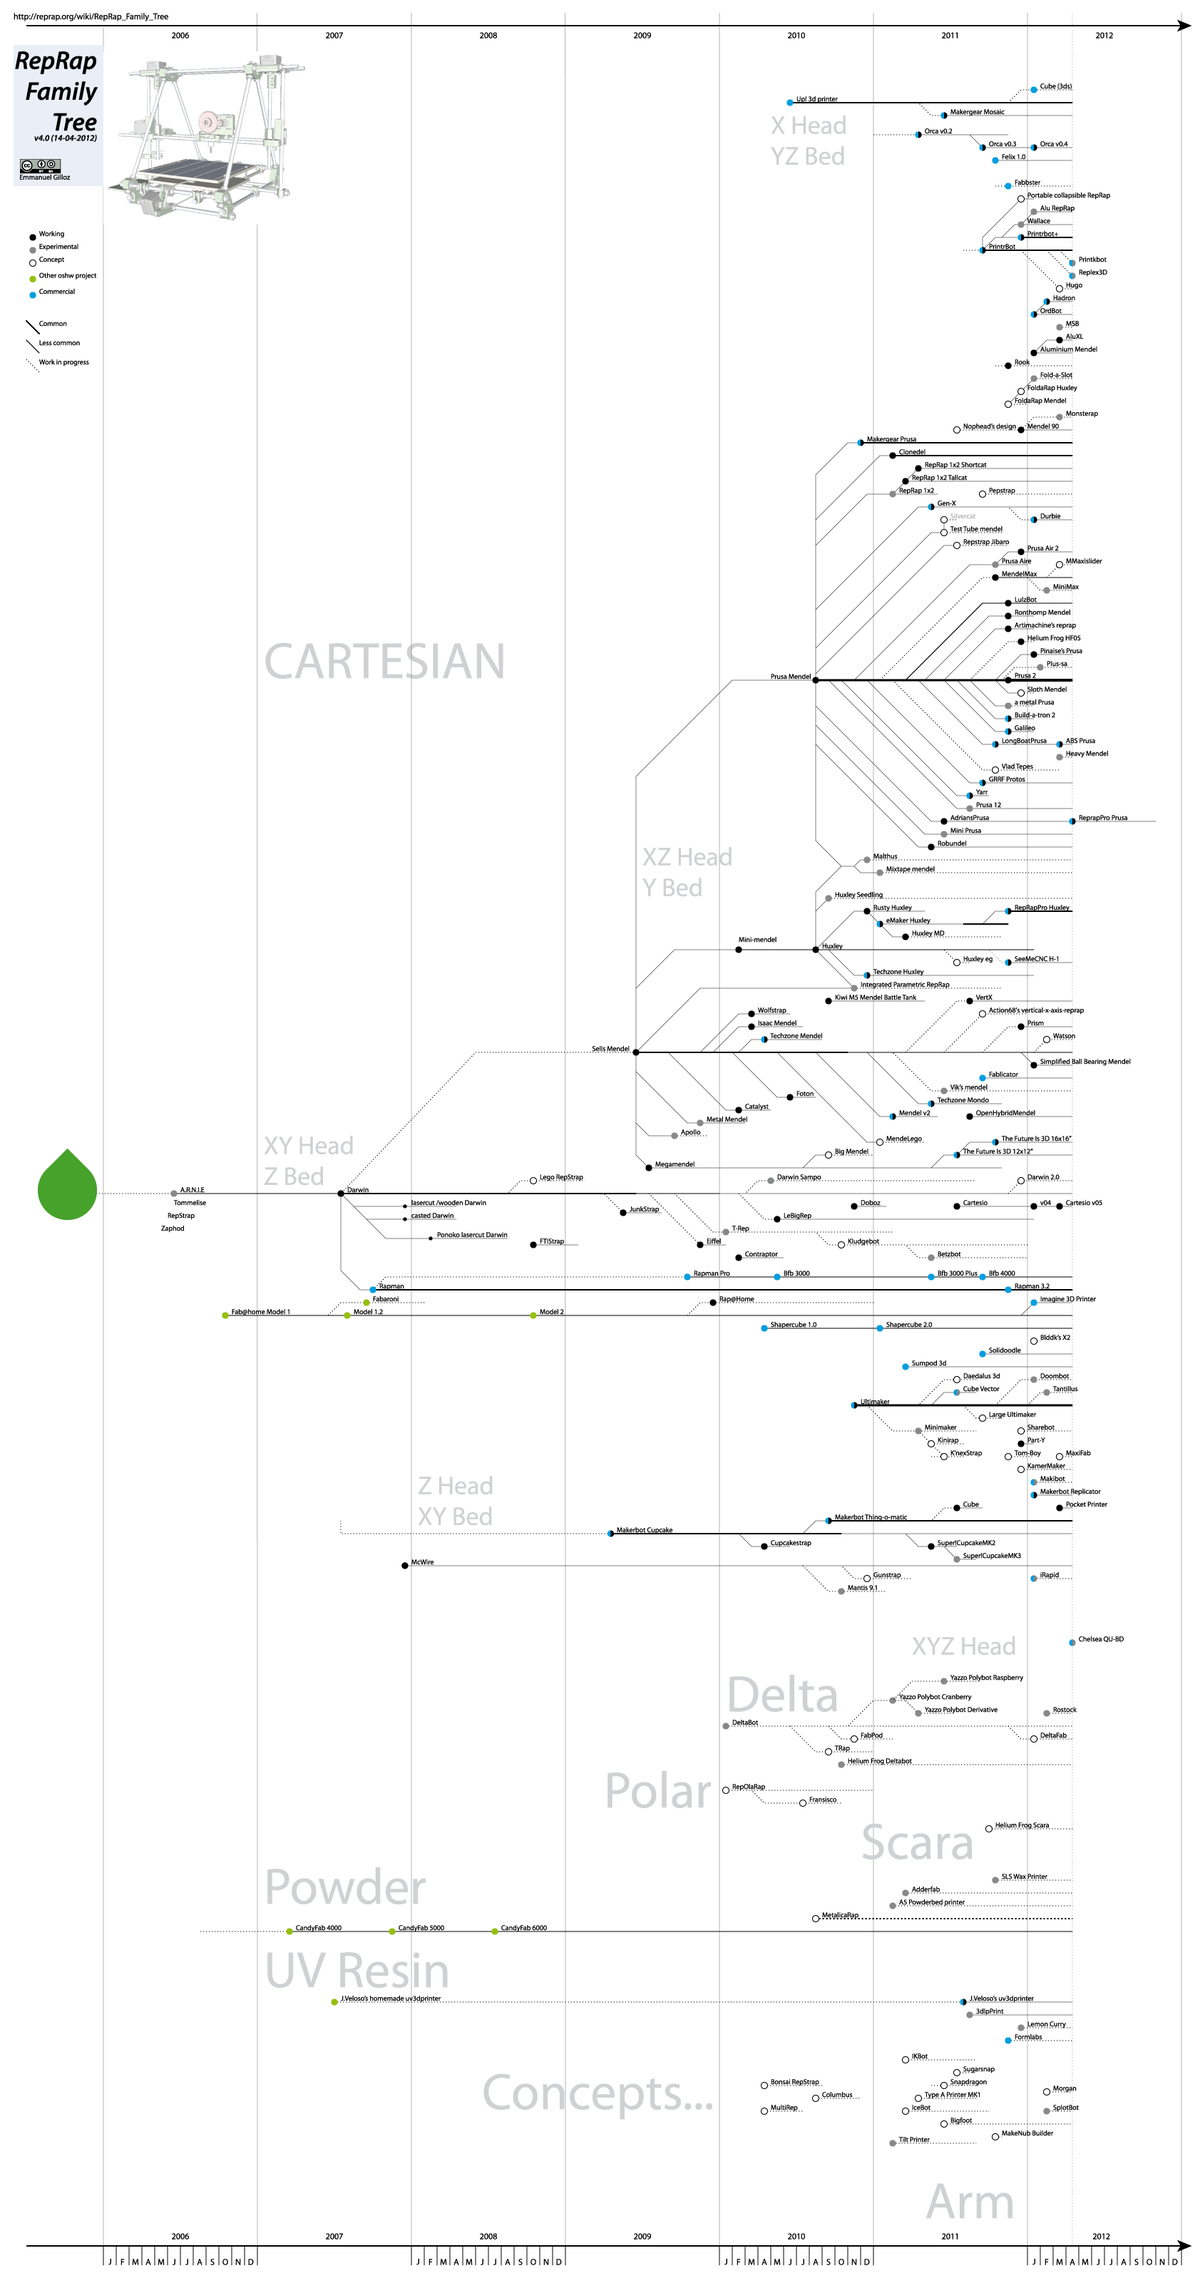
\includegraphics[height=23cm]{reprap_family_tree.png}
    \end{center}
    \caption{Caption here}
    \label{fig:RepRap_family_tree}
\end{figure}



\subsection{A growing movement} % (fold)

Since few years the open hardware movement is growing exponentially,

\begin{figure}[]
    \begin{center}
        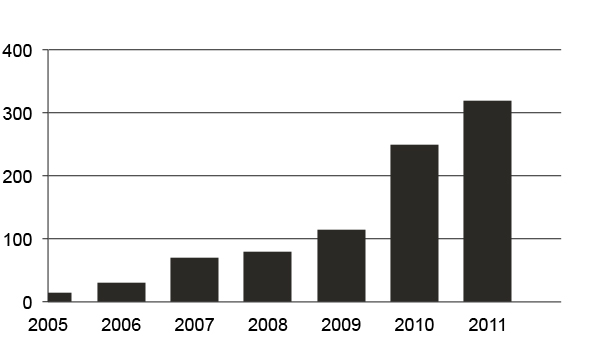
\includegraphics[height=8cm]{oh_project_evolution.jpg}
    \end{center}
    \caption{Creation of new open hardware project per year between 2005 and 2011.
    Graphic extracted from \emph{HOPE 2010 - How to run an open source hardware company}}
    \label{fig:oh_project_evolution}
\end{figure}


\begin{figure}[]
    \begin{center}
        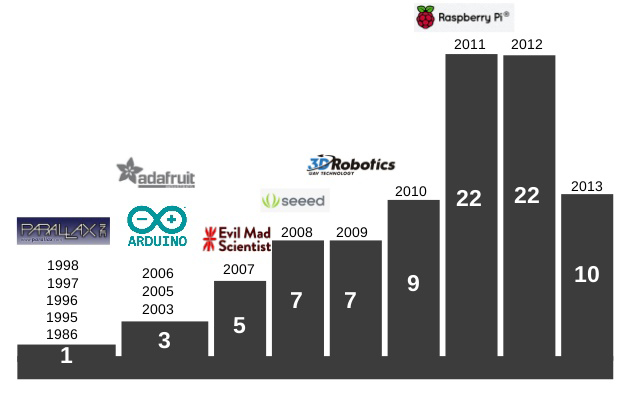
\includegraphics[height=8cm]{oh_startup_creation.jpg}
    \end{center}
    \caption{Start-up creation based on open hardware distribution}
    \label{fig:oh_startup_creation}
\end{figure}

All kind of object begin to have an open source version even the most advanced ones such as laptop (Novena project\footnote{\url{https://www.crowdsupply.com/kosagi/novena-open-laptop}}), reflex camera (OpenReflex\footnote{\url{http://www.instructables.com/id/3D-Printed-Camera-OpenReflex/}}) or even car (LocalMotors\footnote{\url{https://localmotors.com/vehicles/}}, OSVehicle\footnote{\url{http://www.osvehicle.com/}}).



% ref( http://en.wikipedia.org/wiki/Homebrew_Computer_Club, http://www.atariarchives.org/deli/homebrew_and_how_the_apple.php)



\section{Discussion} % (fold)

We have now all the tools needed for real open science and open innovation.

Tesla's Open Source Cars Could Expedite the Growth of the EV Market

These problems occuring in the inventor/entrepreneur world are also the case in research.

The same problem occurs in the research community.
We produce prototype, we need to explore design we do not know how it will works because it is under research.
Acroban was a perfect example, some very good idea such as a multi-articulated column but a realisation handcrafted leading to an impossibility to share our research.
